\documentclass{beamer}
\usetheme{Darmstadt}
\AtBeginSection[]
{
\begin{frame}
    \frametitle{Presentation Outline}
    \tableofcontents[currentsection]
\end{frame}
}
\addtobeamertemplate{navigation symbols}{}
{
\hspace{1em}
\usebeamerfont{footline}%
\insertframenumber / \inserttotalframenumber
}
\setbeamertemplate{caption}[numbered]

\usepackage{graphicx}
\graphicspath{{./tikz/}}
\usepackage{amsmath}
\usepackage{adjustbox}
\usepackage[style=phys, backend=biber]{biblatex}
\renewcommand*{\bibfont}{\scriptsize}
\addbibresource{ref.bib}
\usepackage{caption}
\captionsetup{font=scriptsize}
\usepackage{tcolorbox}
\usepackage{tikz}
\usetikzlibrary{shapes}
\usetikzlibrary{external}
\tikzexternalize

\title{The Worm Algorithm}
\subtitle{physics760: Computational Physics\\Final Project}
\author{Ajay S. Sakthivasan \and Dongjin Suh}
\institute{Universität Bonn}

\date{March 15, 2023}
\begin{document}

\begin{frame}
    \titlepage
\end{frame}

\begin{frame}
    \frametitle{Presentation Outline}
    \tableofcontents
\end{frame}

\section{Introduction}
\begin{frame}{Introduction}
    \begin{itemize}
        \item The Metropolis algorithm is a widely used Monte Carlo method for the Ising model.
        \item The problem of critical slowing down
        \item Prokof’ev and Svistunov proposed an alternative update algorithm called the Worm Algorithm (WA)
        \item WA preserves the local nature of the update step, but achieves a very small dynamical exponent.
    \end{itemize}
\end{frame}

\section{Theoretical Basis}
\subsection{The Ising model}
\begin{itemize}
    \item A mathematical model to understand the behaviour of systems phase transitions, like ferromagnetic materials
    \item 2D Ising model: Magnetic system consisting of interacting spins on a two-dimensional lattice
\end{itemize}
\begin{frame}{The Ising model}

Hamiltonian: 
    \begin{align*}
    H = J\sum_{\langle i,j \rangle} s_{i}s_{j} - h\sum_{i} s_{i}
\end{align*}

Partition function: 
\begin{align*}
    Z = \sum_{s} \mathrm{e}^{-\beta H} = \sum_{s} \mathrm{e}^{-[-\beta J \sum_{\langle i,j \rangle}s_i s_j - \beta h \sum_{i}s_i]}
\end{align*}
\end{frame}

\subsection{Physical observables}
\begin{frame}{Physical observables}
    describe the properties of the system change at phase transition   
    \begin{itemize}
        \item Magnetization 
            \begin{align}
            M = \frac{1}{N}\sum_{i}^{N} \sigma_{i}
            \end{align}
            with N being the amount of sites. For a square lattice, one simply replaces N by $L^{2}$, where L is the lattice length and $\sigma$ the spin. \\
        \item Energy
        \item Autocorrelation - Dynamical Exponent z
             $\tau \approx L^z$ for large $J$ and $\beta$ 
        \item Susceptibility
        \begin{align}
    \chi = (k_B \beta) \cdot (\langle M^2 \rangle-\langle M \rangle^2)
\end{align}
        \item Specific heat
        \begin{align}
    C = (k_B \beta)^2 \cdot (\langle E^2 \rangle-\langle E \rangle^2) 
\end{align}
    \end{itemize}
\end{frame}


\section{Methodology}

\subsection{Metropolis-Hastings Algorithm}
\begin{frame}{Metropolis-Hastings Algorithm}
    \begin{itemize}
        \item Monte Carlo simulation method 
        \item generate samples from a probability distribution
        \item iterative update of the system with the Accept-Reject method
        \item Implement Metropolis-Hastings method
        \begin{enumerate}
            \item Random configuration of an N × N lattice
            \item  Flip the spin at the site
            \item Calculate the energy cost $\Delta$E of the flip
            \item The reject/accept step
        \end{enumerate}
        
    \end{itemize}
\end{frame}

\subsection{The Worm Algorithm}
\begin{frame}{The Worm Algorithm}
\begin{itemize}
    \item The worm algorithm is an alternative to the standard Metropolis algorithm.
\end{itemize}
\end{frame}

\begin{frame}
\begin{itemize}
    \item There are many variations of the worm algorithm in literature.
    \item Our first implementation of the worm algorithm is as follows:
    \begin{enumerate}
        \item Start with an arbitrary lattice configuration.\footnotemark
        \item Select an arbitrary point to create the worm.
        \item Grow the worm: \\
        \begin{enumerate}
            \item Choose a random direction to move.
            \item If the new point is of the same spin as the old point, add it to the worm with probability 1.
            \item If not, perform a Metropolis-like check. If a flip is favourable, flip and add
            \item This way, we create a worm with equal spins.
            \item Break when the worm head meets its tail or if a flip is no longer favourable.
        \end{enumerate}
        \item Measure the observables.
        \item Carry out the desired number of iterations, with a new worm every time.
    \end{enumerate}
    \item There are a few caveats.
\end{itemize}
\footnotetext[1]{We started with an ``almost" cold start.}
\end{frame}

\begin{frame}
\begin{itemize}
    \item Given below is a worm at an intermediate step of its growth.
    \item The lattice below is a small part of the total lattice.
\end{itemize}
\begin{figure}
    \centering
    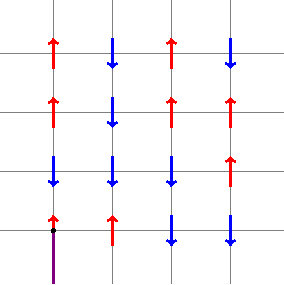
\includegraphics{tikz1.pdf}
\end{figure}
\end{frame}

\begin{frame}
\begin{itemize}
    \item The worm decides to move right.
    \item The new site has the same spin as the old site.
\end{itemize}
\begin{figure}
    \centering
    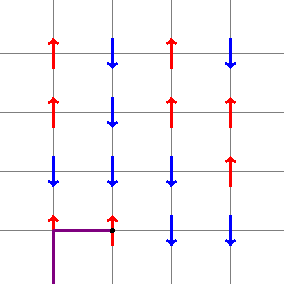
\includegraphics{tikz2.pdf}
\end{figure}
\end{frame}

\begin{frame}
\begin{itemize}
    \item The worm decides to move right.
    \item The new site has the opposite spin as the old site.
    \item Now we perform a metropolis-like check and decide whether to flip or not.
\end{itemize}
\begin{figure}
    \centering
    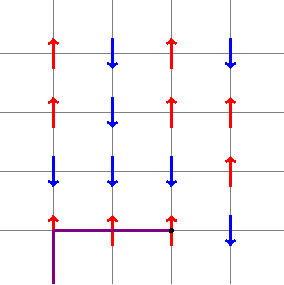
\includegraphics{tikz3.pdf}
\end{figure}
\end{frame}

\begin{frame}
\begin{itemize}
    \item The worm after a few more steps.
\end{itemize}
\begin{figure}
    \centering
    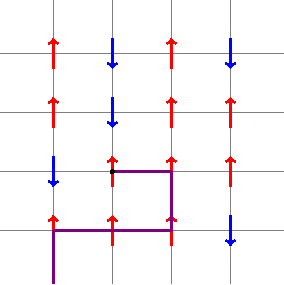
\includegraphics{tikz4.pdf}
\end{figure}
\end{frame}

\begin{frame}
\begin{itemize}
    \item Caveat: If the worm tries to move to a point that is already a part of the worm, we need to update the head accordingly.
    \item We want only an even number of bonds between the sites.
    \item We ensure this by choosing the new head and breaking an old bond appropriately.
\end{itemize}
\begin{columns}
\begin{column}{0.5\textwidth}
\begin{figure}
    \centering
    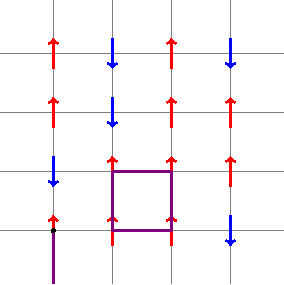
\includegraphics{tikz5.pdf}
\end{figure}
\end{column}
\begin{column}{0.5\textwidth}
\begin{figure}
    \centering
    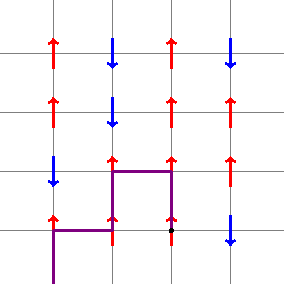
\includegraphics{tikz6.pdf}
\end{figure}
\end{column}
\end{columns}
\end{frame}

\begin{frame}
\begin{itemize}
    \item Caveat: If the worm tries to leave the lattice, let it choose a different dirrection.
\end{itemize}
\end{frame}

\section{Results}
\subsection{Algorithm behavior}
\begin{frame}{Algorithm behavior - Metropolis}
    
\end{frame}
\begin{frame}{Algorithm behavior - Worm Algorithm}
    
\end{frame}

\subsection{Susceptibility and Heat Capacity}
\begin{frame}{Susceptibility and Heat Capacity - Metropolis}
\end{frame}
\begin{frame}{Susceptibility and Heat Capacity - Worm Algorithm}
\end{frame}

\subsection{Autocorrelation time - Dynamical Exponent}
\begin{frame}{Dynamical Critical Exponent - Metropolis}    
\end{frame}
\begin{frame}{Dynamical Critical Exponent - Worm Algorithm}
\end{frame}


\section{Discussion}

\end{document}